\documentclass[11.5pt]{sig-alternate} % sets document style to sig-alternate
% packages
% typesetting
%\usepackage{dirtytalk} % typset quotations easier (\say{stuff})
\usepackage{hanging} % hanging paragraphs
\usepackage[defaultlines=3,all]{nowidow} % avoid widows
\usepackage[pdfpagelabels=false]{hyperref} % produce hypertext links, includes backref and nameref
\usepackage{xurl} % defines url linebreaks, loads url package
\usepackage{microtype}
%\usepackage[super]{nth} % easily create superscript ordinal numbers with \nth{x}
\usepackage{textcomp}
\newcommand{\texttildemid}{\raisebox{0.4ex}{\texttildelow}}
% layout
%\usepackage{enumitem} % control layout of itemize, enumerate, description
\usepackage{fancyhdr} % control page headers and footers
\usepackage{float} % improved interface for floating objects
%\usepackage{multicol} % intermix single and multiple column pages
% language
\usepackage[utf8]{inputenc} % accept different input encodings
\usepackage[english]{babel} % multilanguage support
% misc
\usepackage{graphicx} % builds upon graphics package, \includegraphics
%\usepackage{lastpage} % reference number of pages
%\usepackage{comment} % exclude portions of text (?)
\usepackage{xcolor} % color extensions
\usepackage[backend=biber, style=apa]{biblatex} % sophisticated bibliographies % necessary for HTML to display author info and date on abstract page
\usepackage{csquotes} % advanced quotations, makes biblatex happy
\usepackage{authblk} % support for footnote style author/affiliation
% tables and figures
\usepackage{tabularray}
%\usepackage{array} % extend array and tabular environments
\usepackage{caption} % customize captions in figures and tables (rotating captions, sideways captions, etc)
%\usepackage{cuted} % allow mixing of \onecolumn and \twocolumn on same page
\usepackage{multirow} % create tabular cells spanning multiple rows
%\usepackage{subfigure} % deprecated, support for manipulation of small figures
%\usepackage{tabularx} % extension of tabular with column designator "x", creates paragraph-like column whose width automatically expands
%\usepackage{wrapfig} % allows figures or tables to have text wrapped around them
%\usepackage{booktabs} % better rules
% dummy text
%\usepackage{blindtext} % blind text dummy text
%\usepackage{kantlipsum} % Kant style dummy text
\usepackage{lipsum} %lorem ipsum dummy text
% other helpful packages may be booktabs, longtable, longtabu, microtype

\pagestyle{fancy} % sets pagestyle to fancy for fancy headers and footers

% header and footer
% modern way to set header image
\renewcommand{\headrulewidth}{0pt} % defines thickness of line under header
\renewcommand{\footrulewidth}{0pt} % defines thickness of line above header
\setlength\headheight{80.0pt} % sets height between top margin and header image, effectively moves page contents down
\addtolength{\textheight}{-80.0pt} % seems to affect the lower height. maybe only works properly if footer numbers enabled?
\fancyhf{}
\fancyhead[CE, CO]{
\includegraphics[width=\textwidth]{headerImage.png}}
% footer
%\fancyfoot[LE,LO]{Article Title Here \\ DOI: }% left footer article title and doi
%\fancyfoot[CE,CO]{{}} % center footer empty
%\fancyfoot[RE,RO]{\thepage} % right footer page numbers
%\pagenumbering{arabic} % arabic (1, 2, 3) numbering in footer

\hypersetup{colorlinks=true,urlcolor=blue} % sets link color to blue
\urlstyle{same} % sets url typeface to same as rest of text

% set caption and figure to italics, label bold, left align captions, does not transfer to HTML
\captionsetup{labelfont=bf, font={large, it}, justification=raggedright, singlelinecheck=false}
\renewcommand\theContinuedFloat{\alph{ContinuedFloat}}

%this next bit is confusing, but essentially changes the width of the abstract. Seems to have been copied from this https://tex.stackexchange.com/questions/151583/how-to-adjust-the-width-of-abstract
\let\oldabstract\abstract
\let\oldendabstract\endabstract
\makeatletter %changes @ catcode to enable modification (in parsep)
\renewenvironment{abstract} %alters the abstract environment
{\renewenvironment{quotation}%
               {\list{}{\addtolength{\leftmargin}{1em} % change this value to add or remove length to the the default ?
                        \listparindent 1.5em%
                        \itemindent    \listparindent%
                        \rightmargin   \leftmargin%
                        \parsep        \z@ \@plus\p@}%
                \item\relax}%
               {\endlist}%
\oldabstract}
{\oldendabstract}
\makeatother %changes @ catcode to disable modification

% checks
% italics -
% links -
% dashes -
% tildes -
% dollars - 
\begin{document}

\title{Implications of 3-D Printing for Teaching Geoscience Concepts to Students with Visual Impairments}

\author[1]{\large \color{blue}Karen E. Koehler}
\author[1]{\large \color{blue}Sean Tikkun}
\author[1]{\large \color{blue}Tiffany A. Wild}

\affil[1]{Shawnee State University}
\affil[2]{North Carolina Central University}
\affil[3]{The Ohio State University}

\toappear{}
%% ABSTRACT
\maketitle
\begin{@twocolumnfalse} 
\begin{abstract}
\item 
\textit{This article presents the results of a study on the use of 3-D printed models in a science classroom for students with visual impairments and examines whether the use of these models impacts student conceptual understanding and misconceptions related to geosciences concepts, specifically plate tectonics.}

\textit{Data were collected one week prior to instruction, one week after instruction and throughout the 3-week instructional period. Results showed that students with visual impairments held many of the same misconceptions about plate tectonics as students who are typically sighted. All students in this study had fewer misconceptions after the instructional period than they held before instruction began; however, both the 3D group and the TG group continued to hold approximately equal numbers of misconceptions. The adaptations and hands-on experiences in this 3-week curriculum proved effective for students with visual impairments; helping them understand the unifying theory of plate tectonics.} 

\textit{Some unique misconceptions held by the students with visual impairments in this research study include plates floating on the ocean, earthquakes moving with the plates, and volcanoes working together with the plates to cause earthquakes. There was a difference between students who had low vision and those with light perception only. The study helps to shed light on the use of 3-D printed models in the science classroom and their effectiveness at helping students with visual impairments learn important geoscience concepts.}
\\ \\
Keywords: 3-D printing, visual impairments, conceptual change, misconceptions
\end{abstract}
\end{@twocolumnfalse}

%% AUTHOR INFORMATION

\textbf{*Corresponding Author, Karen E. Koehler}\\
\href{mailto: kkoehler@shawnee.edu }{(kkoehler@shawnee.edu)} \\
\textit{Submitted  Jun 28 2018 }\\
\textit{Accepted Oct 12 2018} \\
\textit{Published online Dec 11th, 2018} \\
\textit{DOI:10.14448/jsesd.10.0004} \\
\pagebreak
\clearpage
\begin{large}
\section*{INTRODUCTION}
The Next Generation Science Standards based upon the National Research Council’s \textit{A Framework for K-12 Science Education: Practices, Crosscutting Concepts, and Core Ideas} stress the need for improved instruction in all areas of science (NRC, 2012). These standards, arranged in a coherent manner and internationally benchmarked, were developed to address the need for a scientifically and technologically literate workforce that could compete on the global scale.  The design of the standards is meant to “help provide students with an organizational framework for connecting knowledge from the various disciplines into a coherent and scientifically based view of the world” (Achieve, 2013).  One area of the standards focuses on instruction in the geosciences across all grade bands including core concepts such as Earth systems - how and why the Earth is constantly changing, the geologic history of the Earth, and the tectonic processes that produce changes in the Earth’s surface at varying time and spatial scales (NRC, 2012).  

An understanding of important geoscience concepts is not only called for in these national standards, but is also important as our society grapples with issues related to energy use and production, geologic natural disasters, and the effects of climate change on our planet and as we prepare the next generation of students to become informed, scientifically literate citizens.  Researchers have called for improved instruction in the geosciences to help students better understand major geologic processes and correct prevalent misconceptions (Libarkin et al., 2005).  

Misconceptions in science occur because a student brings alternative or naïve understandings into the learning situation (Driver and Easley, 1978), which are often very persistent and difficult to change (Chi and Roscoe, 2002).  One area rife with misconceptions is the theory of plate tectonics (Marques and Thompson, 1997; Gobert, 2005; Libarkin, 2005; Libarkin et al., 2005; Sibley, 2005; Ford and Taylor, 2008; Smith and Bermea, 2012) due to the complexity of its underlying processes (Ford and Taylor, 2008; Dolphin, 2008; Smith and Bermea, 2012).  Research shows that sighted middle school students have misconceptions about the composition of tectonic plates, their relationship to ocean basins and continents and their thickness and location on the Earth (AAAS Project 2061, n.d.).  Middle school students also possess many misconceptions about the plate boundaries and the movement at those boundaries (AAAS Project 2061, n.d.; Ford \& Taylor, 2006).  In a study of middle school students, Capps, McAllister \& Boone (2013) also found that they had misconceptions related to the structure of the earth’s interior and the layers of the earth.  Fries-Gaither (2008) also highlighted student misconceptions related to volcanoes and their distribution across the earth’s surface.  She found that students believed that volcanoes only existed on land and were randomly distributed across the earth’s surface.  

Like sighted students, students with visual impairments have difficulty understanding geologic concepts, such as volcanoes, contour and undersea maps, topographic maps and geologic time (Jones et al., 2006) and hold some of the same misconceptions (Koehler et al., 2015); however, research on specific geologic misconceptions held by students with visual impairments is extremely limited.  Students with visual impairments can learn the same science content as their sighted peers (Jones et al, 2006) but will need certain accommodations to make visual material accessible.  It is imperative that these students receive the same preparation for tackling very important societal issues related to the geosciences.   

Researchers have suggested that 3-D printing may hold promise for students with visual impairments to address concept development, provide access to visual information (Horowitz and Schultz, 2014; Koehler et al., 2015; Rosenblum and Herzberg, 2015; Horvath and Cameron, 2016; Jo et al, 2016) and to specifically address science content (Horowitz and Schultz, 2014; Hasper et al., 2015). This article presents the results of a study on the use of 3-D printed models in a science classroom for students with visual impairments and examines whether the use of these models impacts student conceptual understanding and misconceptions related to geosciences concepts, specifically plate tectonics.

\subsection*{Science Instruction and Students with Visual Impairments}

Middle school classrooms often use a wide variety of visual representations to help students understand scientific concepts (i.e. pictures, diagrams, graphs, etc.), which can be problematic for students with visual impairments (Penrod et al., 2006; Jones et al., 2006; Sahin and Yorek, 2009).  In the United States, there are approximately 63,000 children, ages three through twenty-one, with a documented visual impairment (American Printing House, 2017).  This number is based upon polls of state data, used to track the number of students who are legally blind and eligible to receive free reading materials in braille, large print or audio format.   While there is no single definition for blindness, the statutory definition of legal blindness is “when central visual acuity must be 20/200 or less in the better eye with the best possible correction or that the visual field must be 20 degrees or less” (National Federation of the Blind, 2014). However, most states in the United States use the definition of visual impairments set forth in the Individuals with Disabilities Education Act (IDEA, 2004) to define visual impairments as “Visual impairment including blindness means an impairment in vision that, even with correction, adversely affects a child’s educational performance.  The term includes both partial sight and blindness”.  Students with visual impairments are a diverse group of individuals, with varying levels of usable vision and often possess accompanying intellectual and/or physical disabilities.  Students who are blind and visually impaired have a significant sensory loss and perceive the world around them very differently than their sighted peers (Ferrell, 2000).  Because vision plays a major role in access to information, mathematics and science concept development can often pose challenges for students with visual impairments, but with appropriate accommodations, these students can overcome these challenges. 

\subsection*{Tactile Graphics}

Best practice instruction of students with visual impairments calls for the use of tactile graphics to replace visual materials so that students have access to the same content as their sighted peers (Zebehazy and Wilton, 2014b).  Tactile graphics are raised line drawings of pictures, diagrams, charts, graphs, or “graphics intended to be read principally by touch rather than vision” (Aldrich et al., 2003, p. 284).  There is a high variability in production methods of tactile graphics, and the method is not based upon what students prefer, but is based upon cost or ease of production (Smith and Smothers, 2012).  Science textbooks are often produced without tactile graphics; however, even when present, the tactile graphics can pose difficulties for students with visual impairments because they lack detail and quality (Zebehazy and Wilton, 2014a; 2014c).  Sheppard and Aldrich (2001) found that tactile graphics derived from visual graphics often caused information overload and clutter for the student with visual impairments and Zebehazy and Wilton (2014b) found that these graphics did not promote student understanding.  Diagrams and graphs pose problems for students with low vision or no vision because they are only seeing a piece of the diagram or graph at one time and they do not get the” big picture”, whereas students with vision can see the “big picture” at once.  Researchers have expressed concerns regarding the difficulty of students to read and interpret tactile diagrams, especially those attempting to convey concepts of scale or 3-dimensional views of an object (Sheppard and Aldrich, 2001; Bolt and Thurlow, 2004; Andreou and Kotsis, 2005; Kamei-Hannan, 2009).  

\subsection*{3-Dimensional Printing}

Given the limitations of tactile graphics and research by Bolt and Thurlow (2004) indicating that student conceptual understanding might not be indicative of their ability to read a tactile graphic, some have suggested that 3-D printing may hold the key to improving conceptual understanding for students with visual impairments (Horowitz and Schultz, 2014; Koehler et al., 2015; Rosenblum and Herzberg, 2015; Horvath and Cameron, 2016; Jo et al, 2016) and can increase STEM engagement and create accessible curriculum content (Buehler, Comrie, Hofmann, McDonald and Hurst, 2016).  Stangl, Kim and Yeh (2014) reported on the use of 3-D printed picture books for young children for developing emergent literacy skills and creating a community of practice around creating and improving the process of creating these books as an instructional tool for young children.  Götzelmann, Branz, Heidenreich \& Otto (2017) report on their efforts to create an accessible method for individuals who are blind to generate their own 3-D printed objects at home using personal equipment and currently available 3-D designs found on the internet. 

3-D printing traces its roots to the 1950s with the invention of Computer Numeric Controlled (CNC) machines.  CNC machines use lasers and water cutting jets to mill down raw stock material following the instructions on a digital file (Martin et al., 2014).  Today’s 3-D printers use instructions from a digital file, designed using Computer aided design (CAD) software or downloaded from the Internet to extrude very thin layers of heated plastic material to create the 3-dimensional object (Martin et al., 2014).  The New Media Consortium Horizon Report states that 3-D printing will become more prevalent in schools, as the cost of 3-D printers continues to decline (NMC, 2013).  The report outlined many practical uses for 3-D printing technology in educational settings, including STEM related activities and even suggested the use of 3-D printed models for giving access to the visual arts for students with visual impairments, by creating 3-dimensional models of famous works of art.  A recent small-scale study by Jo et al. (2016) reported that 3-D printed models helped students in a Korean school for the blind to grasp concepts in a way that was superior to simply providing a verbal description; however, this study had no control group.  While the use of 3-D printing for helping students with visual impairments learn science concepts has been suggested (Horowitz and Schultz, 2014; Hasper et al., 2015), none of these suggestions are linked to empirical research studies with students with visual impairments.  

The cost of consumer grade 3-D printers has declined; however, they are still a costly alternative to tactile graphics and can sometimes experience print malfunctions due to clogged print heads, operator error or incorrect 3-D print designs.  While the market in 3-D printing has shown significant growth and a number of models are available for as little as \$300, many of these printers do not have the same reliability or build volume as more expensive tools. The leaders in the market have continued to refine their product making them much more approachable to educators with varying degrees of technical knowledge. Tactile models and distinguishing traits require flexibility in build volume to ensure concepts and features are clear, making some of the smaller and inexpensive tools less desirable. The highest scored printer in the category “Best for Schools” in a 2017 annual review was around \$1,000 which seems to be a consistent bench mark in cost (Makezine, 2017). Likewise, there is a steep learning curve when working with some of the common CAD software packages used to create the original design.  However, if 3-D printing is found to be a superior alternative to tactile graphics, the benefits may outweigh the challenges for providing accessibility for student with visual impairments. 

\subsection*{Purpose}

This article presents the results of a study on the use of 3-D printed models in a science classroom for students with visual impairments and examines whether the use of these models impacts student conceptual understanding and misconceptions related to geosciences concepts, specifically plate tectonics.  Additionally, it attempted to uncover the unique misconceptions that students with visual impairments may have about plate tectonics and how those compare to misconceptions held by middle school students without visual impairments.  This was the first study to examine the misconceptions regarding plate tectonics that students with visual impairments hold.  There is a lack of current research on students with visual impairments and their understanding of science concepts (Smothers and Goldston, 2009; Wild and Allen, 2009; Wild, Hilson \& Farrand, 2013) and the findings of this study will add to the growing body of research that seeks to understand how students with visual impairments learn science concepts.  

\section*{THEORETICAL FRAMEWORK}

Conceptual change is a slow, gradual (Vosniadou, 2003), iterative, constructivist process that involves restructuring of prior knowledge (Vosniadou, 2001; Entwistle, 2007) which is heavily influenced by not only the learner’s cognitive processes but also by the cultural and social surroundings (Hatano and Inagaki, 1997).  Conceptual change undergirds much of the research in science instructional methods and student learning in the science classroom.  Producing conceptual shifts in students’ science understanding poses challenges because many science concepts are “complex, dynamic processes” (Chi and Roscoe, 2002).  Inherent in the theoretical framework of conceptual change is the understanding that students often enter the classroom with naïve conceptions, which are scientifically inaccurate and are referred to in the literature as misconceptions (Chi, 1992).  According to Duit and Treagust (2010) many of these misconceptions remain even after instruction takes place and are very resistant to change.  Research finds that students at all grade levels demonstrate many misconceptions related to the earth's interior (Capps et al, 2013) and plate tectonics (Marques and Thompson, 1997; Gobert, 2005; Libarkin and Anderson, 2005; Libarkin et al, 2005; Sibley, 2005; Ford and Taylor, 2008; Smith and Bermea, 2012) preventing them from fully understanding complex geologic processes.  Students with visual impairments possess misconceptions about geology concepts like their sighted peers; however, some misconceptions unique to the students with visual impairments include: people causing Earth’s processes, plates moving due to water pressure; using research or museums to date and reconstruct planetary history; life cycles causing interaction of Earth’s systems, and using water marks to tell about events in Earth’s history (Wild, Hilson \& Farrand, 2013; Koehler, Tikkun \& Wild, 2015).  While there have been numerous studies related to the misconceptions that students with visual impairments hold about scientific ideas history (Wild \& Trundle, 2010b; Wild, Hilson \& Farrand, 2013; Wild, Hilson, \& Hobson, 2013; Koehler, Tikkun \& Wild, 2015), this is the first to examine their in-depth misconceptions related to plate tectonics.  

\section*{METHODS}

This research study examined whether the use of 3D printed objects impacted the conceptual understanding of geologic principles of middle school students who are visually impaired.  Specifically, this study examined if the students’ conceptual understanding of plate tectonics is different when 3D objects are used versus traditional tactile graphics.  The following research questions were investigated:  

 \begin{enumerate}
     \item How do the conceptual understandings of students who use 3D models differ from those that use traditional tactile graphics in the middle school science classroom?
     \item What are the misconceptions that students with visual impairments have about plate tectonics and how do these compare to misconceptions held by middle school students without visual impairments?
 \end{enumerate}

This small scale, qualitative study helped to answer these questions and will add to the growing body of research that seeks to understand how students with visual impairments learn science concepts.  

\subsection*{Setting and Participants}

The participants in this research study were 7th and 8th grade middle school students with visual impairments at a Midwestern specialized school for the blind in the United States.  All instruction took place in a traditionally equipped science classroom.  Specialized schools for the blind, formerly known as residential schools for the blind, typically provide educational services to a variety of students with visual impairments, including those with multiple disabilities.  These schools also provide residential services, in the form of dorm style housing, to students who do not reside in the local community.  This specialized school for the blind provides students with science instruction that meets the state curricular standards in all areas of science and follows the same standardized assessment procedures as a traditional public middle school.  The major differences between this specialized school and a traditional public school is the small student to teacher ratio – typically no more than 8:1, higher levels of individualized instruction and the common use of accommodations and modifications made for both instruction and standardized assessment to meet the unique visual needs of the students. 

Four middle school students, who obtained parental consent, agreed to participate in the study; however, all five students in the middle school classroom received instruction.  Demographic information of the participants is found in Table 1.

\begin{table}[ht]
\caption{Participant demographics}
\begin{tabular}{lll}
\hline
\textbf{Participant} & \textbf{Gender} & \textbf{Visual Acuity} \\ \hline
Molli & Female & Low vision \\
Amber & Female & Light perception only \\
Dennis & Male & Light perception only \\
Yasmine & Female & Low vision \\ \hline
\end{tabular}
\end{table}
  
All names used to identify the participants in this study are pseudonyms.   The researchers separated the students into two groups, the 3-D group and the tactile graphic group, prior to the start of the instructional period and each group was composed of two students.  Each group received the same instruction, but at different times of the day.  This was done to keep the treatment groups separate and to insure that the 3D group only viewed the 3-D printed models and the TG group only viewed the tactile graphics.  One group, identified as the 3-D group (3D), was composed of two girls, one having no light perception and one with low vision.  Low vision is defined as a person who has measurable vision but has difficulty accomplishing or cannot accomplish visual tasks, even with prescribed corrective lenses, but who can enhance his or her ability to accomplish these tasks with the use of compensatory visual strategies (Corn and Lusk, 2010).  Compensatory visual strategies are those skills that help individuals with visual impairments access the core curriculum, which may include:  braille, large print, access to print using optical devices, tactile symbols, etc.  Light perception is defined as a person who can perceive the difference between light and darkness, but has severely reduced vision.  The second group, identified as the tactile graphics group (TG), was composed of one girl with low vision and one boy having no light perception.  The IRB did not allow for collection or reporting on additional demographic information of the participants.  

\subsection*{Materials}
  
Over a three-week instructional period, the primary researcher taught lessons from the inquiry-based instructional series, “Plate Tectonics: The Way the Earth Works” (Cuff, Carmichael and Willard, 2002) from the Great Explorations in Math and Science series from Lawrence Hall of Science.  This researcher, who is a certified science teacher with expertise in teaching students with visual impairments, adapted the lessons for use with students with visual impairments, but the content of the lessons was not altered.  All students received the same instruction from the same instructor, but at different times of the day.  The only difference between the instruction for each treatment group was that the TG group was given tactile graphics demonstrating specific science concepts from the American Printing House’s Basic Science Tactile Graphics booklet or teacher-made graphics and the 3D group was given 3-D printed models of the same science concepts.  The primary choice for the tactile graphics was to use existing, research-based graphics from the American Printing House, when available, because this would lend validity to the materials.  However, not all concepts could be conveyed using pre-existing graphics; therefore, the remainder were designed using best practice tactile graphics design based upon The Braille Authority of North America (BANA, 2011) guidelines.  All 3-D printed models were designed and printed by the third researcher, who is experienced in both 3-D design and 3-D printing, and is a certified teacher of the visually impaired.  This researcher has created numerous 3-D designs, including developing an OpenSCAD braille generator for adding braille elements to 3-D printed designs.  The 3-D printed models, intended to represent certain visual concepts in the plate tectonics curriculum, were designed from scratch using \textit{Google SketchUp}™, a freeware 3-D design program, or modifying open source designs from \textit{Thingiverse}, an open source repository, for 3-D designs affiliated with MakerBot™.  The 3-D designs were printed on a Replicator 2, desktop 3-D printer by MakerBot™.  The models were designed to replicate key instructional photos in the plate tectonics curriculum.  For example, in lesson 2, the students were introduced to the San Andreas fault through discussion of a diagram of the outline of the state of California, with a dashed line indicating the San Andreas fault.  The cities of Los Angeles and San Francisco were labeled in the diagram.   The primary researcher emailed a Pdf of the original diagram to the researcher doing the 3-D design who decided to replicate the original drawing in the 3-D design but to create a groove representing the San Andreas fault.  Once the model was completed, a picture of the model was sent to the primary researcher for approval or suggestions for revision.  Depending upon the complexity of the design, approval and revision of each model varied; however, the entire process of model development and revision took approximately 6 months.  In total, there were four 3-D printed models and four equivalent tactile graphics used in this study.  

\subsection*{The Lessons}
 
During the instructional unit, participants engaged in discussion and hands-on activities designed to provide them with an understanding of the theory of plate tectonics and associated geoscience concepts (Cuff et al., 2002).  The TG group and the 3D group participated in these discussions and hands-on activities at different times of the day, but the instruction and activities were the same for each group and were provided by the same instructor.  The only difference between each treatment group was that the TG group had access to only tactile graphics during the instruction and the 3D group had access to only 3-d printed models during the instruction.   The lessons, adapted from “Plate Tectonics: The Way the Earth Works” and adhering to national science standards, used inquiry-based teaching methods that placed students in the role of scientists, conducting simulated science investigations at field sites around the world.  The lessons helped students generalize what they learned at each field site and apply those findings to the unifying theory that underlies various geosciences phenomena.  Each student received a geologic field notebook at the beginning of the unit, which they used to complete investigations and take data as they moved from one simulated field site to another. The students were very conscientious about bringing their field notebooks to class each day and the notebooks seemed to create a more authentic experience for the students. The instructional unit was broken up into four sessions covering the topics of geologic time and major earth processes that impact the Earth’s surface; faults and their relationship to earthquakes; volcanoes and their relationship to magma viscosity and temperature; and the relationship of earthquakes and volcanoes to tectonic plate boundaries.  An overview of the instructional content in the lessons, the interview questions tied to each lesson and a description of the tactile graphics and 3-D printed model accommodations made for each lesson is found in the \textit{Appendix A}.

\subsubsection*{Session 1}

In the first 2-day session of the plate tectonics curriculum, “Plate Tectonics: The Way the Earth Works” (Cuff et al, 2002), students began by sharing prior knowledge of the structure of the Earth and then made clay models of the sedimentary rock layers found in the Earth’s crust.  They compared these models to the tactile graphics and 3-D printed models of the sedimentary layers, understanding that Earth structures, such as the Grand Canyon, require very long periods of time to form and that this is possible, given the age of the Earth.  They also compared the tactile graphics and 3-D printed models of the 4 major layers of the Earth, understanding that the landforms of the Earth relate to the interaction of these layers (Cuff et al., 2003).

The lesson began with a discussion to elicit student prior knowledge of geology, features of the earth’s crust and tectonic plates and layers of the earth.  The students in the tactile graphics group explored the tactile diagram of the earth’s layers from page 28 of The American Printing House’s Basic Science Tactile Graphics Curriculum (Otto, Poppe and Hayden, 2002) as shown in Figure 1.  
 
\begin{figure}[h]
     \centering
     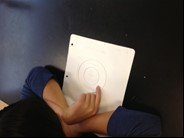
\includegraphics{images/fig1.jpg}
     \caption{Student pointing to tactile diagram of earth’s layers – earth layers seen as concentric circles}
 \end{figure} 
 
The tactile diagram was chosen because it was part of a research based set of tactile graphics from the American Printing House collection of basic science tactile graphics; however, it did not differentiate between the inner and outer core, but included braille labels.   The 3D group explored a 3-D printed model with a cutaway view showing the inner core, outer core, mantle and crust, each layer labeled in braille as seen in Figure 2.  This 3-D printed model closely resembled the cutaway view shown in “Plate Tectonics: The Way the Earth Works” (Cuff et al., 2002). 
   
\begin{figure}[h]
    \centering
    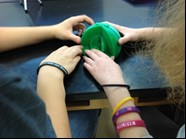
\includegraphics{images/fig2.jpg}
    \caption{Students exploring 3-d printed model of earth’s layers – cutaway view of the earth}
\end{figure}

All students constructed models of layered rock formations using Model Magic® in order to simulate how layers of rock form in the earth’s crust.  They created alternating layers of spheres and pancakes to simulate layers of rock with different characteristics, i.e. sand/soil, boulders, etc.  They were given three minutes to create the first model and five minutes to create a second model and described or drew a picture of each model in their field notebooks.  Students then explored either a tactile diagram of sedimentary rock layers from page 30 of The American Printing House’s Basic Science Tactile Graphics kit (Otto et al., 2002) or a 3-D model of sedimentary rock layers.  The tactile diagram was printed on off-white colored plastic paper, commonly used for tactile graphics production.  Each layer of sedimentary rock was produced using a distinct texture (small circles, dots, zigzags, etc) and this diagram was chosen because it clearly demonstrated the concept of sedimentary rock layers and had been vetted for quality and content validity by researchers, educators and students with visual impairments through APH research.  The tactile graphic was not labeled in either print or braille.  The 3-D printed model of the sedimentary rock layers were made from four different colored stacking blocks of plastic, which had four easily distinguishable raised textures on their front surfaces as shown in Figure 3.
  
\begin{figure}[h]
     \centering
     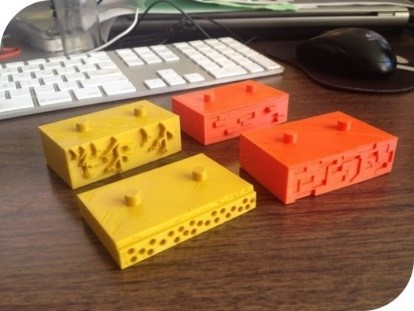
\includegraphics{images/fig3.jpg}
     \caption{3-D printed model of sedimentary rock layers}
 \end{figure} 
 
The textures of the front surface were chosen because they were distinct from one another and were approved by the researchers who were knowledgeable about tactile accommodations for students with visual impairments, but the textures were not tested prior to use in this study. 

Finally, session 1 ended with an exploration of geologic time, in which the students examined a geologic timeline constructed from rope and beads. Each meter length on the timeline, which was marked off with a bead, represented one billion years and the timeline stretched from the present to five billion years ago.  The researcher directed the students to travel back in time while having the students hold onto the rope and then asked them “how old do scientists believe the earth to be?”.  She also directed them to stand at the points on the timeline which they thought best represented when humans first appeared on Earth and when dinosaurs went extinct.  
 
\subsubsection*{Session 2}

During the next 3 days the students “traveled” to California for their first field study.  They put the clay models from session 1 onto “fault simulators” to simulate measurement of displacement of the crust along the San Andreas fault.  Students were introduced to the concept of tectonic plates and discovered the connection between earthquakes and faults and how these are related to tectonic plates and their movement (Cuff et al., 2003).

During Session 2 the researcher led a discussion to elicit prior student knowledge of California and faults.  The students were given either a 3-D printed model of the state of California with braille labels of San Francisco and Los Angeles, shown in Figure 4, and an easily distinguishable San Andreas Fault or a tactile diagram created by the researcher using a PIAF© Tactile Graphics Maker.  
 
\begin{figure}[h]
    \centering
    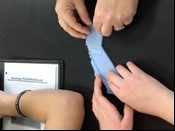
\includegraphics{images/fig4.jpg}
    \caption{ Students exploring 3-d printed model of san andreas fault in California (student is pointing to the groove representing the fault)}
\end{figure}

The tactile diagram showed a raised outline of the state of California with the San Andreas fault labeled with a glitter glue raised line and braille labels for San Francisco and Los Angeles.  Students then worked with fault simulators and the five-minute model of sedimentary rock layers in order to demonstrate the variability of movement along faults, using toothpicks as a simulated fence.  Students measured fence displacement at four simulated fault locations with braille or print centimeter rulers, and calculated and recorded the average fault movement, shown in Figure 5.  
 
\begin{figure}[h]
    \centering
    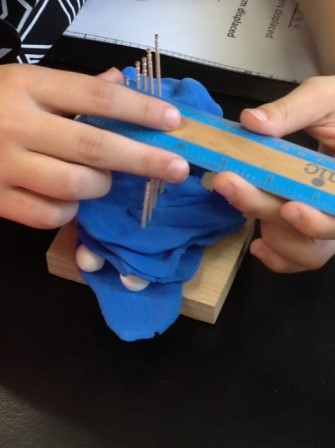
\includegraphics{images/fig5.jpg}
    \caption{Student measuring the displacement of a toothpick fence in clay model of sedimentary rock layers (student using a braille ruler)}
\end{figure}

The researcher led a discussion of plate movement along the San Andreas Fault (attention of the students directed again to the 3-D printed model or the tactile diagram) and discussed the relationship between faults and earthquakes. Students then plotted the location of seven major earthquakes that occurred in 1999 using data from their geologic notebooks.  Students plotted the locations, using the longitude and latitude coordinates, on the World Plotting Map contained in the instructional materials. The researcher enlarged the map on a copier for the two students with low vision and adapted The World at Your Fingers map from The American Printing House for the Blind for the two students with no light perception, shown in Figure 6.  The students with no light perception were able to place foam stickers on the map to indicate locations of earthquakes.  Finally, the students studied their earthquake location maps to look for patterns of earthquake activity.
 
\begin{figure}[h]
      \centering
      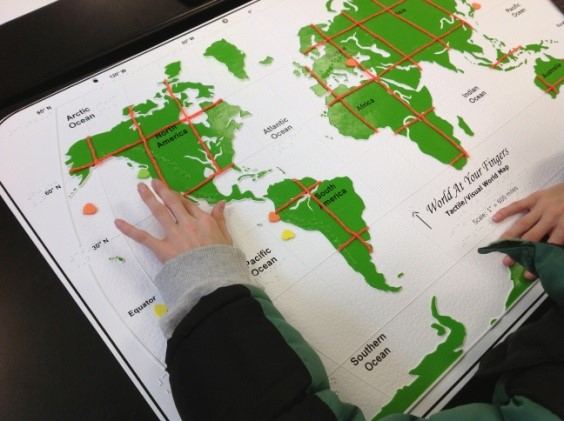
\includegraphics{images/fig6.jpg}
      \caption{Student looking for patterns of plotted earthquakes on the world at your fingers map ©}
  \end{figure}
  
\subsubsection*{Session 3} 

In this 3-day session students used model volcanoes to investigate several important features of Hawaiian shield volcanoes.  Students investigated the eruptions of different “magmas” to explore the relationship between viscosity, temperature, and speed of lava flows.  They learned that the study of shield volcanoes can yield crucial information regarding the nature and composition of the Earth’s upper mantle.  Students then plotted the location of five other shield volcanoes on the world map and noted where they occurred in relation to tectonic plates (Cuff et al., 2003).

During session 3, the students travelled to their second simulated research location in Hawaii to explore shield volcanoes.  The students began by examining tactile graphics of Mauna Loa and Mt. St. Helens and compared and contrasted each volcano.  Next, the students experimented with three different simulated batches of magma to determine the lava flow distance and travel time, to calculate the lava flow velocity, shown in Figure 7.  

\begin{figure}[h]
    \centering
    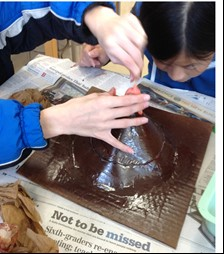
\includegraphics{images/fig7.jpg}
    \caption{Students investigating lava flows using a model volcano – observing simulated lava pouring from the mouth of the volcano}
\end{figure}
 
The simulated batches of magma varied in their viscosity and amount of vinegar.  Students added the same amount of baking soda to each batch of magma, one at a time, to determine lava flow rate.  The students worked in pairs to measure the amount of time it took for each type of lava to travel a predetermined distance from the mouth of the volcano to a raised marker down the slope of the volcano.  Students used the accessible timer on their electronic notetakers or their cellphone to measure the time of eruption and determined the start and stop of the eruption through their ability to feel the foam being released from the mouth of the volcano and then reaching the raised line 1 inch from the bottom of the volcano.  Once the students recorded the lava flow velocities in their field notebooks, they discussed the differences in magma flow viscosity, simulated silica content and magma temperature, as these relate to shield volcano properties.  Finally, the students plotted the location of six major shield volcanoes on their maps in the same manner as they had done for the major earthquakes.  They also looked for patterns related to the location of shield volcanoes around the world.    
  
\subsubsection*{Session 4} 

In this 3-day session, students used model volcanoes to simulate eruptions similar to those of stratovolcanoes found in Japan.  They observed the explosive eruption, and then examined the geographical distribution of stratovolcanoes.  This generated data to help students speculate on the relationship of this type of volcanism to plate tectonics and to the overall structure of the Earth (Cuff et al., 2003).

Session four involved students traveling to their last simulated field site in Japan to explore stratovolcanoes.  Following a discussion of Japan’s location at the edge of the Pacific Plate, the students again experimented with the model volcano to simulate the eruption of a stratovolcano.  A rubber stopper placed in the neck of the volcano represented highly viscous magma, and the stopper popped out, to the delight of the students, as the baking soda and vinegar reaction built up pressure.  The researcher led the students in a discussion of stratovolcanoes and their relationship to subduction zones, showing the students the final tactile diagram or 3-D printed model of a convergent boundary.  The tactile diagram of the convergent boundary was a raised line replica of the original drawing on page 10 of the Geologic Field Notebook materials from the plate tectonics curriculum and depicted the ocean crust sinking under the continental crust and an erupting volcano (Cuff et al., 2003).  The 3-D printed model replicated the original drawing and included a flexible sponge-like material to represent the oceanic crust, which could be manipulated by the student to show the sinking motion of the crust.  The movement of the sponge may have given the students using the 3-D model additional information over the static tactile graphic but the researchers chose to use this to replicate the arrows showing crustal movement on the tactile diagram.  These inquiry-based science lessons were designed to give students a better understanding of the earth as a dynamic, active planet, by allowing them to explore the geologic processes underlying a constantly changing Earth.  

\subsection*{Data Collection}

Qualitative research methods and data collection techniques were chosen because the goal of this research was to uncover how students with visual impairments learn geoscience concepts in the natural setting of the classroom. (Creswell, 2007).  Most data collection in conceptual change research involves some form of pre/post assessment and the use of semi-structur\-ed student interviews to measure pre/post student knowledge has successfully been used in science conceptual change research (Wild, Hilson \& Farrand, 2013; Wild, Hilson \& Hobson, 2013; Wild \& Trundle, 2010b). The co-researcher conducted videotaped interviews one week before the 3-week instructional period and one week after the instructional period.  In addition to the pre/post videotaped interview data, classroom observations, field notes, classroom audio recordings, photographs and student documents were collected throughout the research study period.  The use of multiple data sources for qualitative analysis allowed for uncovering “rich points” which can lead to further analysis of data as themes begin to emerge.  Additionally, the use of multiple data sources in qualitative research provides opportunities for triangulation of data, as the researcher looks across data sources during the analysis phase. Finally, the use of additional data sources beyond the use of a pre/post assessment can aid the researcher in identifying students in the process of conceptual change or uncovering misconceptions.  The co-researcher took field notes and made observations while the primary researcher provided classroom instruction of all science content.  All instructional activities were audiotaped for transcription to ensure fidelity of instruction and to use in a secondary data analysis.  

Student participants were asked seven questions that centered on key concepts from the curriculum and representative questions about geology from the Next Generation Science Standards.  These questions were posed to each participant before and after instruction during individual student interviews. The questions were chosen because they related to concepts in the national standards for middle school geoscience instruction, as well as, state standards related to geoscience concepts.  The major concepts in the interview questions were covered in some way during the 3-week instructional unit as shown in the \textit{Appendix A}.  The seven questions were:  

\begin{enumerate}
     \item How do people date events in Earth’s planetary history? (NRC 2012,  p.177)
     \item How and why is the Earth constantly changing? (NRC, 2012, p.179);
     \item What is the relationship between tectonic plates and the earth’s processes? (Cuff et al., 2003)
     \item Can you tell me what happens here (showing either a tactile graphic or 3-D printed model of fault lines)?  Can you describe what you are showing me?
     \item Can you tell me what the relationship is between tectonic plates and volcanoes?  (Cuff et al., 2003)
     \item How do volcanoes contribute to the recycling of earth materials and energy?
     \item How do living things alter the Earth’s structures and landforms? (NRC, 2012, p.189).
\end{enumerate}
 
Probing questions such as “What do you mean by that concept?” or “So is this what you meant?”  were asked to clarify and further understand the answers from students.  If a student was unsure of the nature of a question, they could ask for follow-up and additional elaboration from the interviewer.  The interviews were digitally recorded and transcribed for analysis.     

\subsection*{Data Analysis}

As the primary researcher, I transcribed all audio and video data, allowing for in-depth understanding of what was happening during the interviews and classroom instruction.  Constant comparative analysis was used to analyze the data (Trundle et al., 2002; Bell and Trundle, 2007; Trundle et al., 2007a; 2007b).  Previous science research exploring conceptual understanding of students with visual impairments (Wild and Trundle, 2010; Wild, Hilson and Farrand, 2013; Wild, Hilson and Hobson, 2013; Hilson, Hobson and Wild, 2016) has successfully employed constant comparative analysis.  The analysis of the interview data, based upon the work of Boeiji (2002), provided a comparison of data collected within a single interview, between interviews in the same group and between interviews in different groups.  This type of comparative analysis was successfully modified and used in conceptual change research by Ucar (2007).  

Prior to analyzing the coded data, an initial coding framework was developed, based upon Next Generation Science Standards and the plate tectonics curriculum (Cuff et al., 2002; NRC, 2012), to establish the criteria needed for a student’s response to be coded as scientific. This initial coding framework was used to differentiate between a scientific understanding and a misconception for use when analyzing data sources.  Following the development of the initial coding framework, the transcribed pre/post interview data were analyzed through the development of a coding framework of understanding based upon the work of Trundle et al. (2007a; 2007b) to categorize students’ learning.  Categories of understanding include: scientific understanding, scientific fragments, scientific with alternative fragments, alternative, alternative with scientific fragments, and no understanding.  Answers coded as scientific must agree with accepted scientific understanding and contain no alternative conceptions.  For an answer to be coded as scientific fragments, it would contain scientific ideas which were incomplete and would not contain any alternative ideas.  Answers coded as scientific with alternative fragments would include a majority of complete scientific understandings but also alternative understandings.  For an answer to be coded as alternative, it must contain only misconceptions and no scientific ideas.  Answers coded as alternative with scientific fragments would include a majority of alternative ideas with at least one scientific understanding.  Finally, in order for an answer to be coded as no understanding the student must show no understanding of the concept, for example this was often the case if the student’s answer was “I don’t know” or “I am not sure”.  Categorization of student understanding in this manner has been used in both conceptual change studies in various content areas, including biology and astronomy and also in studies with students with visual impairments. 

\subsection*{Students’ Categorized Responses}

\subsubsection*{Scientific Responses}
 
In order for students’ responses to be categorized as scientific understanding, the student had to verbalize the following concepts: (1) living things alter the physical characteristics of the Earth (SCI\_LIVING); (2)  evolution impacts the Earth (SCI\_EVOLUTION); (3) sudden changes to the Earth can impact living things (SCI\_SUDDEN); the Earth has tectonic plates (SCI\_PLATES); tectonic plates move (SCI\_MOVE); movement of tectonic plates cause earthquakes (SCI\_EARTHQUAKES); earthquakes happen at faults (SCI\_FAULTS); Movement of tectonic plates causes volcanoes (SCI\_VOLCA\-NOES); movement of tectonic plates causes mountain building (SCI\_MOUNTAINS); rock layers can be used to date Earth’s planetary history (SCI\_LAYERS); fossils can be used to date Earth’s planetary history (SCI\_FOSSILS); volcanoes can recycle earth’s materials and create new rock layers  (SCI\_RECYCLING) (NRC, 2012; Cuff et al., 2002).

The following interview portion provides an example of how the data were coded. 

\begin{quote}

Researcher: Can you tell me what the relationship is between tectonic plates and volcanoes?	

Student: Um…the relationship between them is that when the tectonic plates rub up against each other the oceanic plate goes underneath the continental plate (SCI\_MOVE) and then when it does that it melts and then like heats up the magma and the magma starts to go out of the volcano (SCI\_VOLCANOES)

Researcher: How do volcanoes contribute to the recycling of earth materials and energy?

Student: … When the erupt they um… the lava dries out and cools down and then hardens and makes a new layer of rock (SCI\_RECYLCING)


\end{quote}

\subsubsection*{Students' Misconceptions}

Students with alternative conceptions or misconceptions were those who held beliefs that did not reflect the scientific norms.  Those beliefs were present in both the pre and post interviews in both the 3D group and the TG group.  The following interview excerpts provide an example of how the misconceptions were coded.

\begin{quote}

Researcher: How do people reconstruct and date events in Earth’s planetary history?

Student: They…um..sometimes there are um, like trees they can see if there is like rings on the trees and they see how many rings there are and that counts as years and they can date that back what period that tree came from…(ALT\_TREE RINGS)

Researcher:  How and why is the Earth constantly changing?

Student:  Asteroids (ALT\_ASTEROIDS) falling from the sky and creating craters is the reason that the Earth is constantly changing.
 
Researcher: How do volcanoes contribute to the recycling of earth materials and energy?

Student: Like cups and stuff…um they could make um…pollution and then that pollution would like um…if it was a gas it would be able to seep down into the ground and then it would go into a volcano and then it would mix with the lava (ALT\_Materials)

\end{quote}

The student responses were coded as misconceptions because they did not conform to scientific understandings as reported in the plate tectonics curriculum or the Next Generation Science Standards (NRC, 2012; Cuff et al., 2002). While tree rings can be used to learn about past earth climates and major earth events, the student’s answer above was coded as a misconception because the student’s response did not indicate that they understood how the information from tree rings could be used.  Their answer seemed to indicate that tree rings could only be used to date the age of the tree and determine how long it had existed, which is not appropriate to the question.  Likewise, the idea that asteroids falling from the sky could create constant change on the Earth was not consistent with accepted scientific thought, as these astronomical events are extremely rare.

\subsection*{Trustworthiness}

Member checking was used in this study as defined by Seidman (2006).  Probing questions and clarifying questions were asked of students in order to ensure that researchers were clear on students’ answers.  Additional data were collected in the form of audio recordings, photos of students at work, field notes, and student artifacts to cross-check data and findings during data analysis.  Finally, two researchers on the project worked together to code all the data.  The researchers coded the data simultaneously based upon the coding framework, discussed previously.  When disagreements arose regarding how student responses were coded, discussion ensued until the researchers arrived at a consensus.  At the end of the coding process, the researchers were in 100\% agreement regarding the coded interview data.  

\section*{RESULTS}

The first research question in this study was to examine how conceptual understandings of students who use 3-D printed models differ from those that use traditional tactile graphics in the middle school science classroom.  The students in the 3D group had a total of 8 scientific understandings prior to instruction and 15 scientific understandings after instruction.  The students in the TG group had a total of 8 scientific understandings prior to instruction and a total of 10 scientific understandings after instruction.  All but one student in this study increased their scientific understanding during the 3-week instructional unit as measured by the change in their responses to the interview questions during the pre and post interviews as shown in Table 2.  

\begin{table*}[ht]
\caption{Pre and post results by student and group}
\begin{tabular}{cccc}
\hline
Name & Group & Pre instruction No. of Scientific Understandings & Post Instruction No. of Scientific Understandings \\ \hline
Molli & 3D Printed Model & 3 & 8 \\
Amber & 3D Printed Model & 5 & 7 \\
Dennis & Tactile Graphic & 3 & 3 \\
Yasmine & Tactile Graphic & 5 & 7 \\ \hline
\end{tabular}
\end{table*}

Molli had the greatest increase in scientific understanding and Amber and Yasmine had an equal change in scientific understanding.  The only student who had no change in scientific understandings throughout the unit was Dennis and the student who had the greatest gain in scientific understandings was Molli.  These results were consistent with other data collected during this research.  Dennis used very little scientific language, had many scientific misconceptions and was often very distracted during the lessons.  Molli, on the other hand, significantly increased her scientific understanding during the course of this research study.  She used quite a bit of scientific language, had many fewer misconceptions and was very engaged in our discussions, often taking a leadership role in her group.  The following excerpts from the post-instruction interviews demonstrate the difference discussed above.

\begin{quote}

Researcher:  Can you tell me what the relationship is between tectonic plates and volcanoes?

Molli:  Um… the relationship between them is that when the tectonics plates rub up against each other the oceanic plate goes underneath the continental plate and then when it does that it melts and then like heats up the magma and the magma starts to go out of the volcano.

Researcher:  Can you tell me what the relationship is between tectonic plates and volcanoes?

Dennis:  [grumbles] Volcanoes will erupt.  Tectonic plates will just move but sometimes tectonic plates can cause volcanoes.

Researcher:  Do you know how they do that?

Dennis:  Um… if they hit a really warm place that makes the magma which makes the volcano erupt.  

Researcher:  you say if they hit, what is they?

Dennis:  the plates

Researcher:  so if the plates hit a warm place it causes a volcano?

Dennis:  yeah underground

Researcher:  Oh… underground.  What is that warm place underground?  Do you know?

D:  Its… I think it is the mantle

Researcher: So if a tectonic plate hits the mantle it causes a volcano.  Is that what you are saying?

Dennis:  I think… I don’t know

\end{quote}

While Molli’s understanding is clearly demonstrated and she succinctly explains the relationship between tectonic plates and volcanoes, Dennis struggles to explain his thinking.  He does know that there is a relationship between tectonic plates and volcanoes, and believes that it has something to do with the mantle, but does not demonstrate an understanding of that relationship.  

Overall the students in the 3D group had a gain of +7 in scientific understanding, most of that coming primarily from Molli and the TG group had a gain of +2, wholly coming from Amber.  

\subsection*{Student Misconceptions}

The second research focus in this study was to examine the misconceptions that students with visual impairments have about plate tectonics and how these compare to misconceptions held by middle school students without visual impairments. Researchers have uncovered many misconceptions related to geosciences in students at all levels of schooling.  This research uncovered similar misconceptions held by the participants, both prior to instruction and upon completion of a 3-week unit on plate tectonics.  Overall, the number of misconceptions that the students held was greater pre instruction than post instruction.  The participants held a total of 10 misconceptions prior to instruction and 7 misconceptions after instruction, as shown in Table 3.    

% table 3
\begin{table*}[th]
\caption{Number of misconceptions per group in Pre and Post Interviews}
\begin{tabular}{cccc}
\hline
Group & No. of Misconceptions Pre-interview & No. of Misconceptions Post-Interview & Total \\ \hline
TG & 5 & 4 & 9 \\
3D & 5 & 3 & 8 \\
Total & 10 & 7 & \\ \hline
\end{tabular}
\end{table*}

Both the groups using tactile graphics and the group using 3-D printed models held almost equal numbers of misconceptions, 9 and 8, respectively as shown in Table 3. Each group also held approximately the same number of post instruction misconceptions; the TG group holding 4 misconceptions and the 3D group holding 3 misconceptions as shown in Table 3.  Some of these misconceptions related to the earth systems concepts from the Framework for K-12 Education:  Crosscutting Concepts and Core Ideas (NRC, 2012) which were the focus of some of the pre and post interview questions.  For example, when asked “How and why is the Earth constantly changing”, student responses included:  seasons, Earth’s rotation, canals, asteroids, gravity, and Earth’s orbit.  Misconceptions related to “How the Earth’s planetary history can be dated” included:  tree rings, planetariums and artifacts.  All student misconceptions and their explanations can be found in Appendix A. 

The students held misconceptions throughout the 3-week instructional unit, as evidenced by multiple data sources.  Many of the misconceptions directly related to a misunderstanding of plate tectonics theory and the relationship of these plates to the structure of the earth, as well as the relationship of plate movement to earthquake and volcanic activity.  These findings agree with research done by Smith and Bermea (2012) that found widespread alternative conceptions of plate tectonics in students taking a college level historical geology course.  It is also consistent with previous research demonstrating student misunderstanding of the earth’s layers and internal structure (Libarkin et al., 2005; Sibley, 2005).  Table 4 shows the misconceptions held by the students in the study directly related to the plate tectonics concepts being taught in this unit, as well as the students’ grouping and level of vision.

Many of the students’ misconceptions are the same as those found by Ford and Taylor (2008) in a research project investigating middle school students’ ideas about plate tectonics. In that study, middle school students also described plates as being stacked and described them as being somewhere “down there” and not related to the Earth’s surface; plates can never join and there are gaps between them (Ford and Taylor, 2008).   The misconceptions found in the present study generally fell into three categories:  general understanding of plate tectonics, relationship of plates movement to earthquakes and relationship of plate movement to volcanoes, and the largest number of misconceptions fell into the general understanding category as shown in Table 4. Some student misconceptions uncovered in this study include: plates floating on the ocean, earthquakes moving with the plates, material pollution seeping into a volcano to contribute to Earth’s recycling of materials and volcanoes working together with the plates to cause earthquakes.  These misconceptions have not been reported in existing literature.  

\begin{table*}[!th]
\caption{Category of misconception by group and level of vision}
\begin{tabular}{llll}
\hline
Category of Misconception & Student Explanation & Group & Level of vision (LP or LV) \\
\SetCell[r=7]{h}Plate Understanding & The tectonic plates stack on one another & 3D & LP \\
 & The tectonic plates never touch one another TG & LP \\
 & Tectonic plates underneath volcanoes and earthquakes are moving & TG & LP \\
 & The tectonic plates are separate from the Earth & TG & LP \\
 & Plates are floating on the ocean & TG & LP \\
 & Plates are not under the ocean & LG \& 3D & LP, LV \\
 & The rotation of the Earth explains the relationship between tectonic plates and the Earth & 3D & LP \\
\SetCell[r=4]{h}Relationship of plates to earthquakes & Earthquakes don’t happen in the middle of the ocean & TG \& 3D & LP, LV \\
 & Volcanoes work with plates to create earthquakes & TG & LP \\
 & Earthquakes move with the plates & LG & LP \\
 & There are a lot of earthquakes in Japan because they are right on the fault line of the Pacific plate and the Eurasian plate & TG & LV \\
\SetCell[r=3]{h}Relationship of plates to volcanoes & Pressure from heat given off from the tectonic plates makes the lava clot and the lava explodes and causes a lot of damage. & 3D & LP \\
 & Volcanoes that are around an ocean would be more violent because if they're right next to a plate & 3D & LP \\
 & Where there is a stratovolcano, the plates are right underneath the volcano & 3D & LV \\
\hline
\end{tabular}
\end{table*}

Further analysis of the data seems to indicate that the students with light perception (LP) had far more misconceptions regarding plate tectonics than the students with low vision (LV) and these misconceptions persisted throughout the lessons as evidenced in the post instruction interviews.  Amber and Dennis, both students having only light perception, had the most misconceptions throughout the lessons.   Both Amber and Dennis struggled to understand the idea of plates and their interactions and connection to earthquakes and volcanoes.  This was evidenced in Amber’s classroom documents, when she wrote “I learned that the plates move with the volcanoes and the volcanoes work with the plates to create earthquakes”.  This statement shows that Amber had misconceptions about the structure of plates and their relationship to volcanoes and earthquakes and had little understanding of how interacting plates can produce earthquakes and volcanoes.

Molli and Yasmine were both students with low vision and they had many fewer misconceptions related to plate tectonics than did Dennis and Amber.  Molli and Yasmine together had only four misconceptions but Dennis and Amber together had 12 misconceptions.  Molli and Yasmine appeared to have a greater understanding of the structure of plates and their connection to earthquakes and volcanoes, but each had a unique misconception.  Molli described the relationship between stratovolcanoes and plates as “where there is a stratovolcano the plates are right underneath the volcano”.  Yasmine confused the concept of faults and tectonic plate boundaries when she wrote “there are a lot of earthquakes in Japan because they are right on the fault line of the Pacific plate and the Eurasian plate”.  Finally, all four students initially were surprised to learn that there are plates under the ocean, which is also a misconception reported in previous studies of middle school students (Ford and Taylor, 2008). 

Researchers have pointed to students’ inability to construct mental models of the Earth’s internal structure which impedes their understanding of important fundamental but abstract concepts of plate movement (Gobert, 2005; Libarkin and Baker, 2007; Libarkin and Clark, 2008).  An understanding of plate tectonics theory is at the heart of understanding the cause of earthquakes and volcanoes, however, research shows that middle school students have difficulty conceptualizing the movement of the plates because they are so large, move so slowly and much of the evidence of the internal workings of the Earth cannot be observed (Ford and Taylor, 2008).   The students with visual impairments in this research study also had similar difficulty conceptualizing tectonic plates and their movements, resulting in misconceptions similar to those expressed by students who are sighted.

\section*{DISCUSSION}

This study sought to understand how students with visual impairments learn concepts related to geologic processes, especially plate tectonics, and to help determine if the use of 3-D printed models can help students learn science concepts.  The research also sought to uncover the misconceptions that students with visual impairments hold about plate tectonics and other geoscience concepts and compare these misconceptions to those held by students without visual impairments.  

This study found that all but one of the participants increased their scientific understanding of plate tectonics and associated geoscience concepts throughout the 3-week instructional period, when using an inquiry based curriculum. The students in the 3D group had greater gains in conceptual understanding that the students in the TG group.  All students in this study had fewer misconceptions after the instructional period than they held before instruction began, however, both the 3D group and the TG group continued to hold approximately equal numbers of misconceptions.  

This research shows that students with visual impairments hold many of the same misconceptions about plate tectonics as students who are sighted.  These misconceptions include plates being stacked and not related to the Earth’s surface, as well as plates never being joined and gaps existing between the plates (Ford and Taylor, 2008). These misconceptions are prevalent because of the abstract and complex nature of plate tectonics and the fact that students are unable to witness the action of the plates because of their extremely slow movement.  Some unique misconceptions held by the students with visual impairments in this research study include plates floating on the ocean, earthquakes moving with the plates, and volcanoes working together with the plates to cause earthquakes.  These middle school students, like others who are not visually impaired, bring many naïve conceptions or misconceptions into the science classroom and it is the role of the instructor to help students recognize and change these misconceptions.  

While it may not be possible to attribute the differences in conceptual understanding and misconceptions between the 3D and TG groups to the use of 3-D printed models, there were definite differences in the ways that the students interacted with these instructional tools.  When students in the TG were asked to explore and explain the tactile graphic of the earth layers, they simply read off the names of the layers which were written in braille.  However, when students in the 3D group were asked the same thing, they pointed to and correctly identified each layer.  These students were able to physically dismantle the layers of the earth and clearly differentiate its major layers.  For example, one student pulled apart the model and differentiated each part – the inner core, the outer core, the mantle and the crust.  Additionally, students could reassemble the layers – unlike in the tactile diagram. For example, in Amber’s description, she even commented on the relative size of the mantle as related to the other layers.  

Students using the 3D printed model of the San Andreas fault immediately recognized the long groove as representing the fault but not all students were able to correctly explain what happens at the fault.  One of the students using the tactile diagram, initially, could not distinguish the fault from the outline of the state, but during the post interview was able to find the fault.  

Overall, there were distinct differences in the way that the students interacted with the 3D models than with the tactile graphics.  When examining the 3-D printed models, Amber and Molli spent more time inspecting them and manipulating them – turning them in many different directions to get more information.  Some of this may have been due to the novelty of having models versus tactile graphics, which they confront very frequently.  Dennis and Yasmine, in the tactile graphic group often just read the Braille and spent much less time exploring the graphic.  I frequently had to prompt them to explore all parts of the tactile graphic, often scaffolding their instruction.  

It should be noted that there was a significant difference between students who had low vision and those with light perception only.  The students who had some amount of vision and could see the tactile graphics or 3-D printed models had significantly fewer misconceptions.  It is possible the lack of vision may have impeded the students’ ability to formulate a mental model of important plate features and interactions and caused them to have more misconceptions than the students who had low vision. 

\subsection*{Limitations}

One limitation of the study is the small sample size.  While small sample sizes are normally found in research on students with visual impairments, this limits the generalizability of research done on this population.  While there were clear differences between the two groups, there were too few students to determine if it was indeed the models that led to differences in conceptual understanding or whether there were other factors at play.  Each of the four students had varying levels of vision, but due to the stipulations in the research protocol, additional data related to academic performance, eye disorders and additional disabilities could not be obtained.  Additionally, past instruction in science may also have varied because most of the students were previously educated in different geographical areas of the state, prior to enrolling in this specialized school for the blind.  This limits the ability to draw conclusions about the effectiveness of the 3-D printed models in altering students’ conceptual understandings and reducing misconceptions.  It also limits the transferability of these findings to other educational settings for students with visual impairments.  

\subsection*{Implications}

Results from this study add to the body of research on middle school students’ conceptual understandings and misconceptions of geologic processes related to plate tectonics.  Additionally, it provides preliminary information about the misconceptions that are unique to students with visual impairments.  It also helps to shed light on the use of 3-D printed models in the science classroom and their effectiveness at helping students with visual impairments learn important geoscience concepts.  Traditionally, tactile graphics are used to give students with visual impairments access to visual content; however, with 3-D printing technology becoming more affordable and more widely available, many have suggested 3-D printed models as a superior alternative.  The preliminary results of this study indicate that 3-D printing technology may hold promise for helping students with visual impairments in the science classroom and other curricular areas as well.  This was the first empirical study to examine the effectiveness of using 3-D printed models versus tactile graphics in the science classroom for students with visual impairments.  More research certainly needs to be done, in a variety of science content areas, to determine if 3-D printed models are a more powerful instructional tool than traditional tactile graphics.  Additional research is warranted and it would be beneficial to replicate the study with additional students, both in specialized schools for the blind and those in the general education setting.  As this study was the first of its kind, the results are promising and future research is warranted.    

\end{large}
\clearpage

\section*{REFERENCES}\par 
\leftskip 0.25in
\parindent -0.25in 

Achieve. 2013. Next generation science standards: Achieve, Inc. on behalf of the twenty-six states and partners that collaborated on the NGSS. Available at \url{http://www.nextgenscience.org/} (Accessed 9 October 2016).

Aldrich, F., Sheppard, L., and Hindle, Y. 2003. First steps towards a model of tactile graphicacy. Cartographic Journal, 40:283–287.

American Printing House for the Blind Annual Report (APH, 2017).  Distribution of eligible students based on the federal quota census data (Fiscal Year 2017). Available at \url{https://www.aph.org/files/annual-reports/APH-Annual-Report-FY17.pdf} (Accessed 2 October 2018).

Andreou, Y., and Kotsis, K.  2005. Mathematical concept development in blind and sighted children.  International Journal of Learning, 12:255-260.

Bolt, S. E., and Thurlow, M. L. 2004. Five of the most frequently allowed testing accommodations in state policy: Synthesis of research. Remedial and Special Education, 25:141-152.

Bell, R. L., \& Trundle, K. C. 2008. The use of a computer simulation to promote scientific conceptions of moon phases.  Journal of Research in Science Teaching, 45:346-372.

Buehler, W., Comrie, N., Hofmann, M., McDonald, S., and Hurst, A. 2016. Investigating the Implications of 3D Printing in Special Education. ACM Trans. Access. Comput. 8, 3, Article 11 (March 2016), 28 pages. DOI=\url{http://dx.doi.org/10.1145/2870640}

Braille Authority of North America. 2011. Guidelines and standards for tactile graphics.  Retrieved September 28, 2016, from \url{http://brailleauthority.org/tg/web-manual/}.

Capps, D.K., McAllister, M. and Boone, W.J. 2013.  Alternative conceptions concerning the earth’s interior exhibited by honduran students. Journal of Geosciences Education, 61:231-239.   

Chi, M.T.H. 1992. Conceptual change within and across ontological categories:  Examples from learning and discovery in science. In Giere, R.N., ed., Cognitive models in science.  Minneapolis, MN:  University of Minnesota Press, p. 129–186.

Chi, M.T.H and Roscoe, R.D. 2002.  The processes and challenges of conceptual change. In Limon, M. and Mason, L., eds., Reconsidering conceptual change. Dordrecht, The Netherlands:  Kluwer Academic Publishers, p. 3 – 27.

Corn, A.L. and Lusk, K.E. 2010.  Perspectives on low vision.  In Corn, A. and Erin, J., eds., Foundations of low vision:  Clinical and functional perspectives. New York, NY: AFB Press, p. 3-34.

Creswell, J.W. 2007. Qualitative inquiry and research design:  Choosing among five approaches. Thousand Oaks, CA: Sage.

Cuff, K., Carmichael, I., and Willard, C. 2003.  Plate tectonics: The way the earth works. Lawrence Hall of Science, University of California at Berkeley.

Dolphin, G. 2008. Evolution of the theory of the earth: A contextualized approach for teaching the history of the theory of plate tectonics to ninth grade students. Science and Education: Contributions from History, Philosophy and Sociology of Science and Mathematics, 18:425-441.

Driver, R., and Easley, J. 1978.  Pupils and paradigms:  A review of literature related to concept development in adolescent science students.  Studies in Science Education, 5:61-84.

Duit, R. and Treagust, D.F. 2010. Conceptual change: A powerful framework for improving science teaching and learning. International Journal of Science Education, 25:671-688.

Entwistle, N. 2007.  Conceptions of learning and the experience of understanding: Thresholds, contextual influences, and knowledge objects. In Vosniadou ,S., Baltas, A. and Vamvakoussi, X., eds., Reframing the conceptual change approach in learning and instruction.  Kidlington, Oxford:  Elsevier Science Ltd, p. 123-143.

Ferrell, K. A. (2000). Growth and development of young children. In Holbrook, M. C. and Koenig, A. J., eds., Foundations of education. Volume I: History and theory of teaching children and youths with visual impairments.  New York: American Foundation for the Blind, p. 111 – 134.

Ford, B., and Taylor, M. 2008. Investigating students' ideas about plate tectonics. Science Scope, 30:38.

Fries-Gaither, J. (2008). Common misconception about weathering, erosion, volcanoes, and earthquakes.  Earth’s Changing Surface. Retrieved from \url{http://beyondpenguins.nsdl.org/issue/column.php?date=December2008&departmentid=professional&columnid=professional!misconceptions}

Gobert, J.D. 2005.  The effects of different learning tasks on model-building in plate tectonics:  Diagraming versus explaining.  Journal of Geosciences Education, 53:444-455.

Götzelmann, T., Branz, L., Heidenreich, C., and Otto, M. 2017. A Personal Computer-based Approach for 3D Printing Accessible to Blind People. In Proceedings of the 10th International Conference on Pervasive Technologies Related to Assistive Environments (PETRA '17). ACM, New York, NY, USA, 1-4. DOI: \url{https://doi.org/10.1145/3056540.3064954}

Hasper, E., Windhorst, R.A., Hedgpeth, E., Tuyl, L.V.., Gonzales, A., Martinez, B., Yu, H., Farkas, Z., and Baluch, Z.P. 2015.  Methods for creating and evaluating 3d tactile images to reach stem courses to the visually impaired, Journal of College Science Teaching, 44: 92-99.

Hatano, G., and Inagaki, K. 1997. Qualitative changes in intuitive biology. European Journal of Psychology of Education, 12:111–130.

Hilson, M., Hobson, S., and Wild, T. 2016. Conceptual understandings of students with visual impairments about biodiversity across ecosystems. Journal of Blindness Innovation and Research, 6(2). Available at \url{https://nfb.org/images/nfb/publications/jbir/jbir16/jbir060204.html}. doi: \url{http://dx.doi.org/10.5241/6-102}.

Horowitz, S. and Schultz, P. H.  2014.  Printing Space: Using 3d printing of digital terrain models in geosciences education and research.  Journal of Geoscience Education, 62:138-145.

Horvath, J., and Cameron, R. 2016.  Teaching blind students with 3-d prints [Web log post].  Available at \url{https://blogs.scientificamerican.com/guest-blog/teaching-blind-students-with-3-d-prints/}  (accessed 9 November 2016).

Individuals with Disabilities Education Improvement Act of 2004, Pub. L. No. 108-446, 118 Stat. 2647 (2004).

Jo, W., I, J.E., Harianto, R.A., So, J.H., Lee, H., Lee, H.J., and Moon, M-W. 2016. Introduction of 3d printing technology in the classroom for visually impaired students. Journal of Visual Impairment and Blindness, 110:S115-121. 

Jones, M.G., Minogue, J., Oppewal, T., Cook, M.P., and Broadwell, B. 2006. Visualizing without vision at the microscale:  Students with visual impairments explore cells with touch.  Journal of Science Education and Technology, 15:345–351.

Kamei-Hannan, C. 2009. Innovative solutions for words with emphasis: Alternative methods of braille transcription. Journal of Visual Impairment and Blindness, 103:709-721.

Koehler, K., Tikkun, S.R., and Wild, T.A. 2015.  Impact of 3d printing on conceptual understandings of students with visual impairments. Presentation at the Council for Exceptional Children Conference, San Diego, California.

Libarkin, J.C.  2005.  Conceptions, cognition, and change: Student thinking about the Earth.  Journal of Geoscience Education, 53(4), Editorial.

Libarkin, J., and Anderson, S. 2005. Assessment of learning in entry-level geoscience courses:  Results of the geoscience concept inventory.  Journal of Geoscience Education, 53:394–401

Libarkin, J.C., Anderson, S.W., Dahl, J., Beilfuss, M., and Boone, W. 2005. Qualitative analysis of college students' ideas about the Earth, Interviews and open-ended questionnaires: Journal of Geoscience Education, 53:17-26.

Libarkin, J.C., and Baker, K.M. 2007. Analysis of student conceptions of global
earthquake and volcano occurrence. Abstracts with Programs, Geological Society of America, 39:578.

Libarkin, J., and Clark, S. 2008. The relationship between students’ confidence and conceptual understanding of plate tectonics. Abstracts with Programs, Geological Society of America, 40:421–422.

Marques, L., and Thompson, D. 1997. Misconceptions and conceptual changes 
concerning continental drift and plate tectonics among portuguese students aged 16-17. Research in Science and Technological Education, 15:195-222.

Martin, R. L., Bowden, N. S., and Merrill, C. 2014. 3d printing in technology and engineering education. Technology and Engineering Teacher, 73:30-35.

National Federation of the Blind (NFB). 2014.  Blindness Statistics. Available at   https://nfb.org/blindness-statistics (accessed 4 March 2016).

National Research Council and National Academies Press (2012).   A Framework for K-12 Science Education: Practices, Crosscutting Concepts and Core Ideas.  National Academies Press.

New Media Consortium., 2013.  NMC Horizon Report.  Available at \url{http://www.nmc.org/publications/2013-horizon-report-k12}. (accessed 10 January 2015). 

Otto, F., Poppe, T. and Hayden, F. 2002.  Basic science tactile graphics.  Louisville:  American Printing House.

Penrod, W.M, Haley, C.D., and Matheson, L.P. 2006.  A model for improving science teaching for students with visual impairments.  RE:view, 37:3-58.

Rosenblum, L.P. and Herzberg, T. S. 2015.  Braille and tactile graphics:  Youths with visual impairments share their experiences.  Journal of Visual Impairments and Blindness, 109: 173-184.  

Sahin, M., and Yorek, N., 2009, Teaching science to visually impaired students: A smallscale qualitative study: US-China Education Review, 6:19–26.

Seidman, I. 2006. Interviewing as qualitative research: A guide for researchers in education and the social sciences.  New York: Teachers College Press.

Sheppard, L and Aldrich, F.K. 2001.  Tactile graphics in school education:  Perspectives from teachers.  British Journal of Visual Impairment, 19:93-97.  DOI: 10.1177/\\026461960101900303

Sibley, D.F. 2005.  Visual abilities and misconceptions about plate tectonics.  Journal of Geoscience Education, 53:471-477.

Smith, G.A and Bermea, S. B. 2012.  Using students’ sketches to recognize alternative conceptions about plate tectonics persisting from prior instruction.  Journal of Geoscience Education, 60:350-359.

Smith, D.W. and Smothers, S.M. 2012. The role and characteristics of tactile graphics in secondary mathematics and science books. Journal of Visual Impairment and Blindness, 9:543-544.  

Smothers, S. M., and Goldston, M. J. 2009. Atoms, elements, molecules and matter: An investigation into the congenitally blind adolescents' conceptual frameworks on the nature of matter. Science Education, 94:448-477.

Stangl, A., Kim, J., and Yeh, T. 2014. 3D printed tactile picture books for children with visual impairments: a design probe. In Proceedings of the 2014 conference on Interaction design and children (IDC '14). ACM, New York, NY, USA, 321-324. DOI: \url{http://dx.doi.org/10.1145/2593968.2610482}

Trundle, K., Atwood, R., and Christopher, J.  2002.  Preservice elementary teachers’ conception of moon phases before and after instruction.  Journal of Research in Science Teaching 39:633-658.

Trundle, K., Atwood, R., and Christopher, J.  2007a.  Fourth-grade elementary students’ conception of standards-based lunar concepts.  International Journal of Science Education, 29:595-616.

Trundle, K., Atwood, R., and Christopher, J. 2007b.  A longitudinal study of conceptual change:  Preservice elementary teachers’ conceptions of moon phases.  International Journal of Research in Science Teaching, 44:303-326.

Vosniadou, S. 2001.  What can persuasion research tell us about conceptual change that we did not already know?  International Journal of Educational Research, 35:731-737.

Vosniadou, S. 2003. Exploring the relationships between conceptual change and intentional learning.  In Sinatra, G.M. and Pintrich, P.R., Eds., Intentional conceptual change. Mahwah:  Erlbaum, p. 377–406.

Wild, T. and Allen, A. 2009. Policy analysis of science-based best practices for students with visual impairments.  Journal of Visual Impairments and Blindness, 103:113-116.

Wild, T and Trundle, K. 2010b.  Conceptual understandings of seasonal change 
by middle school students with visual impairments. Journal of Visual Impairment and Blindness, 104:107-108. 

Wild, T., Hilson, M., and Farrand, K.  2013.  Conceptual understanding of 
geological concepts by students with visual impairments.  Journal of Geoscience Education, 61:222-230.

Wild, T., Hilson, M., Hobson, S.  2013.  Conceptual understandings of sound by elementary students with visual impairments.  Journal of Visual Impairment and Blindness, 107:107-116.

Zebehazy, K. T., and Wilton, A. P. 2014a. Quality, importance, and instruction: the perspectives of teachers of students with visual impairments on graphics use by students. Journal of Visual Impairment and Blindness, 108:5-16.

Zebehazy, K. T., and Wilton, A. P. 2014b. Charting Success: The experience of teachers of students with visual impairments in promoting student use of graphics. Journal of Visual Impairment and Blindness, 108:263-274.

Zebehazy, K. T., and Wilton, A. P. 2014c. Straight from the source: Perceptions of students with visual impairments about graphic use. Journal of Visual Impairment and Blindness, 108:275-286.
\clearpage
\leftskip 0in
\parindent 0in 

\begin{table*}[th]
\caption*{\textbf{Appendix A:} Overview of curriculum, interview questions and accommodations}
\begin{tabular}{llllll}
\hline
Lesson Number and Topics & Tactile graphics & Description of Tactile Graphic & 3-D printed models & Description of 3-D printed models & Interview Questions \\ \hline
\begin{tabular}[x]{@{}l@{}} 1 – Geologic Time and Earth Processes \\ geologic time and energy needed to shape the Earth’s surface, natural processes that change and shape the earth’s surface, modeling earth layers and sedimentary rock layers, clues geologists use to understand what happened in the past \end{tabular} 
& \begin{tabular}[x]{@{}l@{}} Tactile graphic of Earth’s layers \#28 in APH Basic Science Tactile Graphics book (Otto et al., 2002) \\ Tactile graphics of sedimentary rock layers \#30 in APH Basic Science Tactile Graphics book (Otto et al., 2002) \end{tabular} 
& \begin{tabular}[x]{@{}l@{}} Raised line graphic with concentric circles representing core, mantle and crust. \\ Raised line graphic with four sedimentary layers represented by various designs (i.e. circles, zigzags, etc) \end{tabular} 
& \begin{tabular}[x]{@{}l@{}} 3-D Earth layer Model based on page 54 of Plate Tectonics: The Way the Earth Works (Cuff et al, 2002) \\ 3-D model of sedimentary rock layers based on page 27 of Plate Tectonics: The Way the Earth Works (Cuff et al, 2002) \end{tabular} 
& \begin{tabular}[x]{@{}l@{}} Spherical 3-D model with cutaway depicting inner core, outer core, mantle and crust \\ Four distinctly textured interlocking blocks representing layers of sedimentary rock. \end{tabular} 
& \begin{tabular}[x]{@{}l@{}} How do people date events in Earth’s planetary history? (NRC 2012, p. 177) \\ How and why is the Earth constantly changing? (NRC, 2012, p.179) \\ How do living things alter the Earth’s structures and landforms? (NRC, 2012, p.189). \end{tabular}  \\
2 – \begin{tabular}[x]{@{}l@{}} Field Work in California \\ Investigating faults,  modeling fault movement tectonic plates and earthquakes, mapping earthquakes around the world \end{tabular} 
& Tactile Graphic of Map of California and San Andreas fault- page 34 Plate Tectonics: The Way the Earth Works (Cuff et al, 2002) – created using PIAF© 
& Raised outline of the state of California with the San Andreas Fault line represented by a dashed raised line 
& 3-D model of Map of California and San Andreas fault based page 34 of Plate Tectonics: The Way the Earth Works (Cuff et al, 2002) 
& Plastic model approximately 1 centimeter thick in the shape of California.  A deep groove representing the San Andreas Fault. 
& \begin{tabular}[x]{@{}l@{}} How and why is the Earth constantly changing? (NRC, 2012, p.179); \\ What is the relationship between tectonic plates and the earth’s processes? \\ Can you tell me what happens here (showing either a tactile graphic or 3-D printed model of fault lines)?  Can you describe what you are showing me? \end{tabular} \\
\begin{tabular}[x]{@{}l@{}} 3–Field Work in Hawaii \\ tectonic plates and shield volcanoes, modeling lava flow, hot spots in mantle, mapping shield volcanoes around the world, recycling of earth materials in shield volcanoes \end{tabular} 
& \begin{tabular}[x]{@{}l@{}}Tactile graphic of Shield vs. stratovolcanos - created using PIAF© \\ Tactile graphic of side view of volcano \#29 in APH Basic Science Tactile Graphics book (Otto et al., 2002) \end{tabular} 
& \begin{tabular}[x]{@{}l@{}}Raised drawings of shield and stratovolcanoes using swell paper \\ Raised line drawing of an erupting volcano \end{tabular} 
& \begin{tabular}[x]{@{}l@{}} 3-D models constructed using papier mache. \\ 3-D model of side view of volcano on page 61 of Plate Tectonics: The Way the Earth Works (Cuff et al, 2002) \end{tabular} 
& \begin{tabular}[x]{@{}l@{}} No 3-D printed model \\ Model of a volcano with a cut-away view on one side, and a center rod that could be pushed up and out of the top of the volcano to simulate an exploding volcano \end{tabular} 
& \begin{tabular}[x]{@{}l@{}} How and why is the Earth constantly changing? (NRC, 2012, p.179); \\ What is the relationship between tectonic plates and the earth’s processes? \\ Can you tell me what the relationship is between tectonic plates and volcanoes? \\ How do volcanoes contribute to the recycling of earth materials and energy? \end{tabular} \\
\begin{tabular}[x]{@{}l@{}} 4 – Field Work in Japan \\ tectonic plates and stratovolcanoes and modeling subduction zones, mapping stratovolcanoes around the world, recycling of earth materials in strato volcanoes. \end{tabular} 
& \begin{tabular}[x]{@{}l@{}} Tactile graphic of Shield vs stratovolcanos using PIAF© \\ Tactile graphic of convergent boundary with subduction zone page 10 of field notebook in Plate Tectonics: The Way the Earth Works (Cuff et al, 2002) –created using Piaf© \end{tabular} 
& Raised drawings of shield and stratovolcanoes using swell paper 
& \begin{tabular}[x]{@{}l@{}}3D models constructed using papier mache. \\ 3-D model of convergent boundary with subduction zone based upon page 10 of Plate Tectonics: The Way the Earth Works (Cuff et al, 2002) \end{tabular} 
& \begin{tabular}[x]{@{}l@{}}No 3-D printed model \\ Convergent boundary model had a rough pad that could be slipped between the two layers of the model.  The pad represented the oceanic crust slipping beneath the continental crust. \end{tabular} 
& \begin{tabular}[x]{@{}l@{}} How and why is the Earth constantly changing? (NRC, 2012, p.179); \\ What is the relationship between tectonic plates and the earth’s processes? \\ Can you tell me what the relationship is between tectonic plates and volcanoes? \\ How do volcanoes contribute to the recycling of earth materials and energy? \end{tabular} \\ \hline
\end{tabular}
\end{table*}

\begin{table*}[th]
\caption*{\textbf{Appendix B:} Misconceptions and explanations of geologic concepts}
\begin{tabular}{ll}
\hline
\textbf{Misconception} & \textbf{Explanation} \\ \hline
Tree rings & Earth’s planetary history can be dated with the use of tree rings \\
Seasons & Seasons are the reason for the constant changing of the Earth \\
Rotation & The rotation of the Earth explains the relationship between tectonic plates and the Earth \\
Stacking & The tectonic plates stack on one another \\
Canals & People building canals account for the reason that the Earth is constantly changing \\
Pressure & Pressure causes rocks and water to get heated in a volcano \\
Asteroids & Asteroids falling from the sky and creating craters is the reason that the Earth is constantly changing \\
Gravity & The gravity on Earth causes it to constantly change \\
Society & Artifacts from people can be used to reconstruct Earth’s planetary history \\
Orbit & The orbit of the Earth causes the Earth to constantly change \\
Plates & The tectonic plates never touch one another \\
Existence & If living things did not exist on Earth there would be no planet Earth \\
Materials & Material pollution (ex. Cups) seep into a volcano and contribute to the recycling of Earth’s materials \\
Planetarium & Planetariums allow for dating and reconstruction of Earth’s planetary history \\
Underneath & Tectonic plates underneath volcanoes and earthquakes are moving \\
Mountains & Earthquakes cause mountains \\
Separate & The tectonic plates are separate from the Earth \\ \hline
\end{tabular}
\end{table*}

\end{document}